\chapter{Filters and Interceptors}
\label{filters_and_interceptors}

Filters and entity interceptors can be registered for execution at well-defined extension points in \jaxrs\ implementations. They are used to extend an implementation in order to provide capabilities such as logging, confidentiality, authentication, entity compression, etc. 

\section{Introduction}
\label{introduction_filters}
Entity interceptors wrap around a method invocation at a specific extension point. 
Filters execute code at an extension point but without wrapping a method invocation.  There are three extension points for filters: Pre, PreMatch and Post. There are two extension points for entity interceptors: ReadFrom and WriteTo.  For each of these extension points, there is a corresponding interface:

\begin{listing}{1}
public interface RequestFilter {
    void preFilter(FilterContext ctx) throws IOException;
}
public interface ResponseFilter {
    void postFilter(FilterContext ctx) throws IOException;
}
public interface PreMatchRequestFilter {
    void preMatchFilter(FilterContext ctx) throws IOException;
}
\end{listing}

\begin{listing}{1}
public interface ReaderInterceptor<T> {
    T aroundReadFrom(ReaderInterceptorContext<T> context) 
        throws IOException, WebApplicationException;
}
public interface WriterInterceptor<T> {
    void aroundWriteTo(WriterInterceptorContext<T> context) 
        throws IOException, WebApplicationException;
}
\end{listing}

A filter is a class that implements \RequestFilter, \PreMatchRequestFilter\ or \ResponseFilter\ (or any combination thereof) and is annotated with \Provider. An entity interceptor is a class that implements \ReaderInterceptor\ or \WriterInterceptor\ (or both) and is annotated with \Provider. 

In the Client API, a \RequestFilter\ is executed as part of the invocation pipeline, before the HTTP request is delivered to the network; still in the Client API, a \ResponseFilter\ is executed upon receiving a server response, before control is returned to the application. 
In the Server API, a \RequestFilter\ is executed upon receiving a request from a client, before the resource method is called (but after it has been matched); still in the Server API, a \ResponseFilter\ is executed as part of the response pipeline, before the HTTP response is delivered to the network.

An entity interceptor implementing \ReaderInterceptor\ wraps around calls to \code{MessageBodyReader} method \code{readFrom}. An entity interceptor implementing \WriterInterceptor\ wraps around calls to \code{MessageBodyWriter} method \code{writeTo}. \jaxrs\ implementations are REQUIRED to call registered interceptors when mapping representations to Java types and vice versa. See Section \ref{entity_providers} for more information on entity providers.

\section{Filters}
\label{filters}

A filter implements one or more of the following interfaces:  \RequestFilter, \PreMatchRequestFilter\ and \ResponseFilter. There is a \emph{filter chain} for each kind of filter. Filters in a chain are sorted based on their priorities (see Section \ref{priorities}) and are executed in order. 


The following example shows an implementation of a logging filter: each method simply logs the message and returns.

\begin{listing}{1}
@Provider
class LoggingFilter implements RequestFilter, ResponseFilter {

    @Override
    public void preFilter(FilterContext ctx) throws IOException {
        logRequest(ctx.getRequest());
    }

    @Override
    public void postFilter(FilterContext ctx) throws IOException {
        logResponse(ctx.getResponse());
    }
    ...
}
\end{listing}

A \FilterContext\ provides access to the request, the response (in response filters) as well as the ability to create and set new responses.

Request filters implementing \RequestFilter\ or \PreMatchRequestFilter\ can implicitly stop the execution of their corresponding chains by setting a response in their associated context. If a response is set by a filter of this type, implementations are REQUIRED to abort execution of the chain and treat the response object as if produced by calling the resource method (Server API) or by executing the HTTP invocation (Client API). For example, upon a cache hit, a client {\em caching} filter may set a response object in the context to optimize network access.

Filters that implement \PreMatchRequestFilter\ are supported only as part of the Server API and are executed upon receiving a client request but {\em before} a resource method is matched. Thus, a pre-match filter has the ability to modify the input to the matching algorithm (see Section~\ref{request_matching}) and, consequently, alter its outcome. 

The following example uses a pre-match filter in order to tunnel requests via POST by using the X-HTTP-Method-Override header to overwrite the HTTP method prior to resource matching.

\begin{listing}{1}
@Provider
class PostMethodOverrideFilter implements PreMatchRequestFilter {

  @Override
  public void preMatchFilter(FilterContext context) throws IOException {
    Request request = context.getRequest();
        
    if (request.getMethod().equalsIgnoreCase("POST")) {
      String m = request.getHeaders().getHeader("X-HTTP-Method-Override");
      if (m != null) {
        request = context.getRequestBuilder().method(m).build();
        context.setRequest(request);
      }
    }
  }
}
\end{listing}

\section{Entity Interceptors}

An entity interceptor implements interface \ReaderInterceptor\ or \WriterInterceptor\ or both. There is an \emph{interceptor chain} for each kind of entity interceptor. Entity interceptors in a chain are sorted based on their priorities (see Section \ref{priorities}) and are executed in order. 

Entity interceptors wrap calls to the methods \code{readFrom} in classes implementing \code{MessageBodyReader} and \code{writeTo} in classes implementing \code{MessageBodyWriter}. An implementation of an interceptor SHOULD explicitly call the context method \code{proceed} to continue the execution of the chain. Because of their wrapping nature, failure to call this method will prevent execution of the wrapped method in the corresponding message body reader or message body writer.

The following example shows an implementation of a GZIP entity interceptor that provides deflate and inflate capabilities~\footnote{This class is not intended to be a complete implementation of this interceptor.}.

\begin{listing}{1}
@Provider
class GzipWidgetInterceptor implements 
    ReaderInterceptor<Widget>, WriterInterceptor<Widget> {

    @Override
    Widget aroundReadFrom(ReaderInterceptorContext<Widget> ctx) ... {
        InputStream old = ctx.getInputStream();
        ctx.setInputStream(new GZIPInputStream(old));
        try {
            return ctx.proceed();
        } finally {
            ctx.setInputStream(old);
        }
    }

    @Override
    void aroundWriteTo(WriterInterceptorContext<Widget> context) ... {
        OutputStream old = ctx.getOutputStream();
        GZIPOutputStream gzipOutputStream = new GZIPOutputStream(old);
        ctx.setOutputStream(gzipOutputStream);
        try {
            ctx.proceed();
        } finally {
            gzipOutputStream.finish();
            ctx.setOutputStream(old);
        }
    }
    ...
}
\end{listing}

The context types, \ReaderInterceptorContext\ and \WriterInterceptorContext, provide read and write access to the parameters of the corresponding wrapped methods. In the example shown above, the input and output streams are wrapped and updated in the context object before proceeding. \jaxrs\ implementations MUST use the last parameter values set in the context object when calling the wrapped methods \code{MessageBodyReader.readFrom} and \code{MessageBodyWrite.writeTo}.

\section{Lifecycle}

By default, just like all the other providers, a single instance of each filter or entity interceptor is instantiated for each \jaxrs\ application. First the constructor is called, then any requested dependencies are injected, then the appropriate methods are called (simultaneously) as needed. Implementations MAY offer alternative lifecycle options beyond the default one. See Section \ref{lifecycle_and_environment} for additional information.

\section{Binding}

Binding is the process by which a filter or interceptor is associated with a resource class or method (Server API) or an invocation (Client API). The forms of binding presented in the next sections are only supported as part of the Server API. See Section \ref{binding_in_client_api} for binding in the Client API.

\subsection{Global Binding}
\label{global_binding}

Global binding is the default type of binding. A filter or interceptor that is only annotated with \Provider\ is bound globally, i.e.~its applicability is all the resource methods in an application. For example, the \code{LoggingFilter} defined in Section \ref{filters} is bound globally. If this filter is part of an application, requests and responses will be logged for all resource methods. 

\subsection{Name Binding}
\label{Name_Binding}

A filter or interceptor can be associated with a resource class or method by declaring a new \emph{binding} annotation \`{a} la CDI~\cite{jsr299}. These annotations are declared using the \jaxrs\ meta-annotation \NameBinding\ and are used to decorate both the filter (or interceptor) and the resource method or resource class. For example, the \code{LoggingFilter} defined in Section \ref{filters} can be bound to the method \code{hello} in \code{MyResourceClass}, instead of globally, as follows:

\begin{listing}{1}
@Provider
@Logged
class LoggingFilter implements RequestFilter, ResponseFilter {
    ...
}
\end{listing}

\begin{listing}{1}
@Path("/")
public class MyResourceClass {
    @Logged
    @GET
    @Produces("text/plain")
    @Path("{name}")
    public String hello(@PathParam("name") String name) {
        return "Hello " + name;
    }
}
\end{listing}

According to the semantics of \code{LoggingFilter}, the request will be logged before the \code{hello} method is called and the response will be logged after it returns. The declaration of the \code{@Logged} annotation is shown next.

\begin{listing}{1}
@NameBinding
@Target({ ElementType.TYPE, ElementType.METHOD })
@Retention(value = RetentionPolicy.RUNTIME)
public @interface Logged { }
\end{listing}

Binding annotations that decorate resource classes apply to all the resource methods defined in them. A filter or interceptor class can be decorated with multiple binding annotations. Similarly, a resource method can be decorated with multiple binding annotations.  Each binding annotation instance in a resource method denotes a set of filters and interceptors whose class definitions are decorated with that annotation (possibly among others). The final set of (static) filters and interceptors is the union of all these sets \footnote{By definition of {\em set}, any duplicate filters or interceptors in each individual set or the final set are eliminated.}; this set must be sorted based on priorities as explained in Section \ref{priorities}. 

\subsection{Dynamic Binding}

The annotation-based forms of binding presented thus far are {\em static}.  By having a filter or interceptor implement the \DynamicBinding\ interface, {\em dynamic} variants of name binding and global binding are possible. In these cases, binding is determined based on (i) the filter or interceptor being associated to a resource method globally or by name and (ii) the value returned by the \code{isBound} method in \DynamicBinding. 

The following example defines a global \code{LoggingFilter} that is bound dynamically to all resource methods in \code{MyResourceClass} that are annotated with \code{@GET}.

\begin{listing}{1}
@Provider
class LoggingFilter implements RequestFilter, DynamicBinding {

    public boolean isBound(Class<?> type, Method method) {
        return type.equals(MyResourceClass.class) 
            && method.isAnnotationPresent(GET.class);    
    }
    ...
}
\end{listing}

\jaxrs\ implementations SHOULD resolve dynamic binding filters and interceptors at most once for each resource method (typically at deployment time).

\subsection{Binding in Client API}
\label{binding_in_client_api}

Binding in the Client API is accomplished via API calls instead of annotations. \Client, \Invocation, \InvocationBuilder\ and \Target\ are all configurable types: their configuration can be accessed by calling the \code{configure} method. See Sections \ref{configurable_types} for more information.

\section{Priorities}
\label{priorities}

The order in which filters or interceptors are executed as part of their corresponding chains is controlled by the \BindingPriority\ annotation.
Priorities are represented by integer numbers. All execution chains except
for the Post chain are sorted in ascending order; the lower the number the higher the priority. The Post filter chain is sorted in descending order to ensure that response filters are executed in {\em reverse order}.

The \code{BindingPriority} class defines a set of built-in priorities for security, header decorators, decoders and encoders. The default binding priority is \code{BindingPriority.USER}. For example, the priority of an authentication filter can be set as follows:

\begin{listing}{1}
@Provider
@Authenticated
@BindingPriority(BindingPriority.SECURITY)
public class AuthenticationFilter implements RequestFilter {
    ...
}
\end{listing}

Note that even though, as explained in Section \ref{binding_in_client_api}, annotations are not used for binding in the Client API, they are still used to define priorities. Therefore, if a priority other than the default is required, the \BindingPriority\ annotation must be used for a filter or interceptor registered using the Client API. 

The order in which filters and interceptors that belong to the same priority class are executed is implementation dependent.

\section{Exceptions}
\label{exceptions_filters_and_interceptors}

When a filter or interceptor method throws an exception, the \jaxrs\ runtime will attempt to map the exception as described in Section \ref{exceptions_providers}.  As explained in Section \ref{exceptionmapper}, an application can supply exception mapping providers to customize this mapping.

\section{Relationship between Filters and Interceptors}

As stated above, filters and entity interceptors are used to extend an implementation in order to provide capabilities such as logging, security, etc. Filters have access to the complete message and can be used for multiple purposes. However, any task that involves transforming a message entity is likely better suited for an entity interceptor. 

It is worth mentioning that an interceptor may be triggered by a filter that reads (or writes) an entity. This is 
because filters may trigger message body readers (or writers) and these may, in turn, be wrapped by reader (or writer) interceptors. Figure \ref{jaxrs_pipeline} depicts this relationship. 

Figure \ref{jaxrs_pipeline} also shows the relationship between pre-match filters and entity interceptors: namely, given that these type of filters are executed before matching, only interceptors bound globally wrap calls to the message body readers and writers in this case.

\begin{figure}[H]
\centering
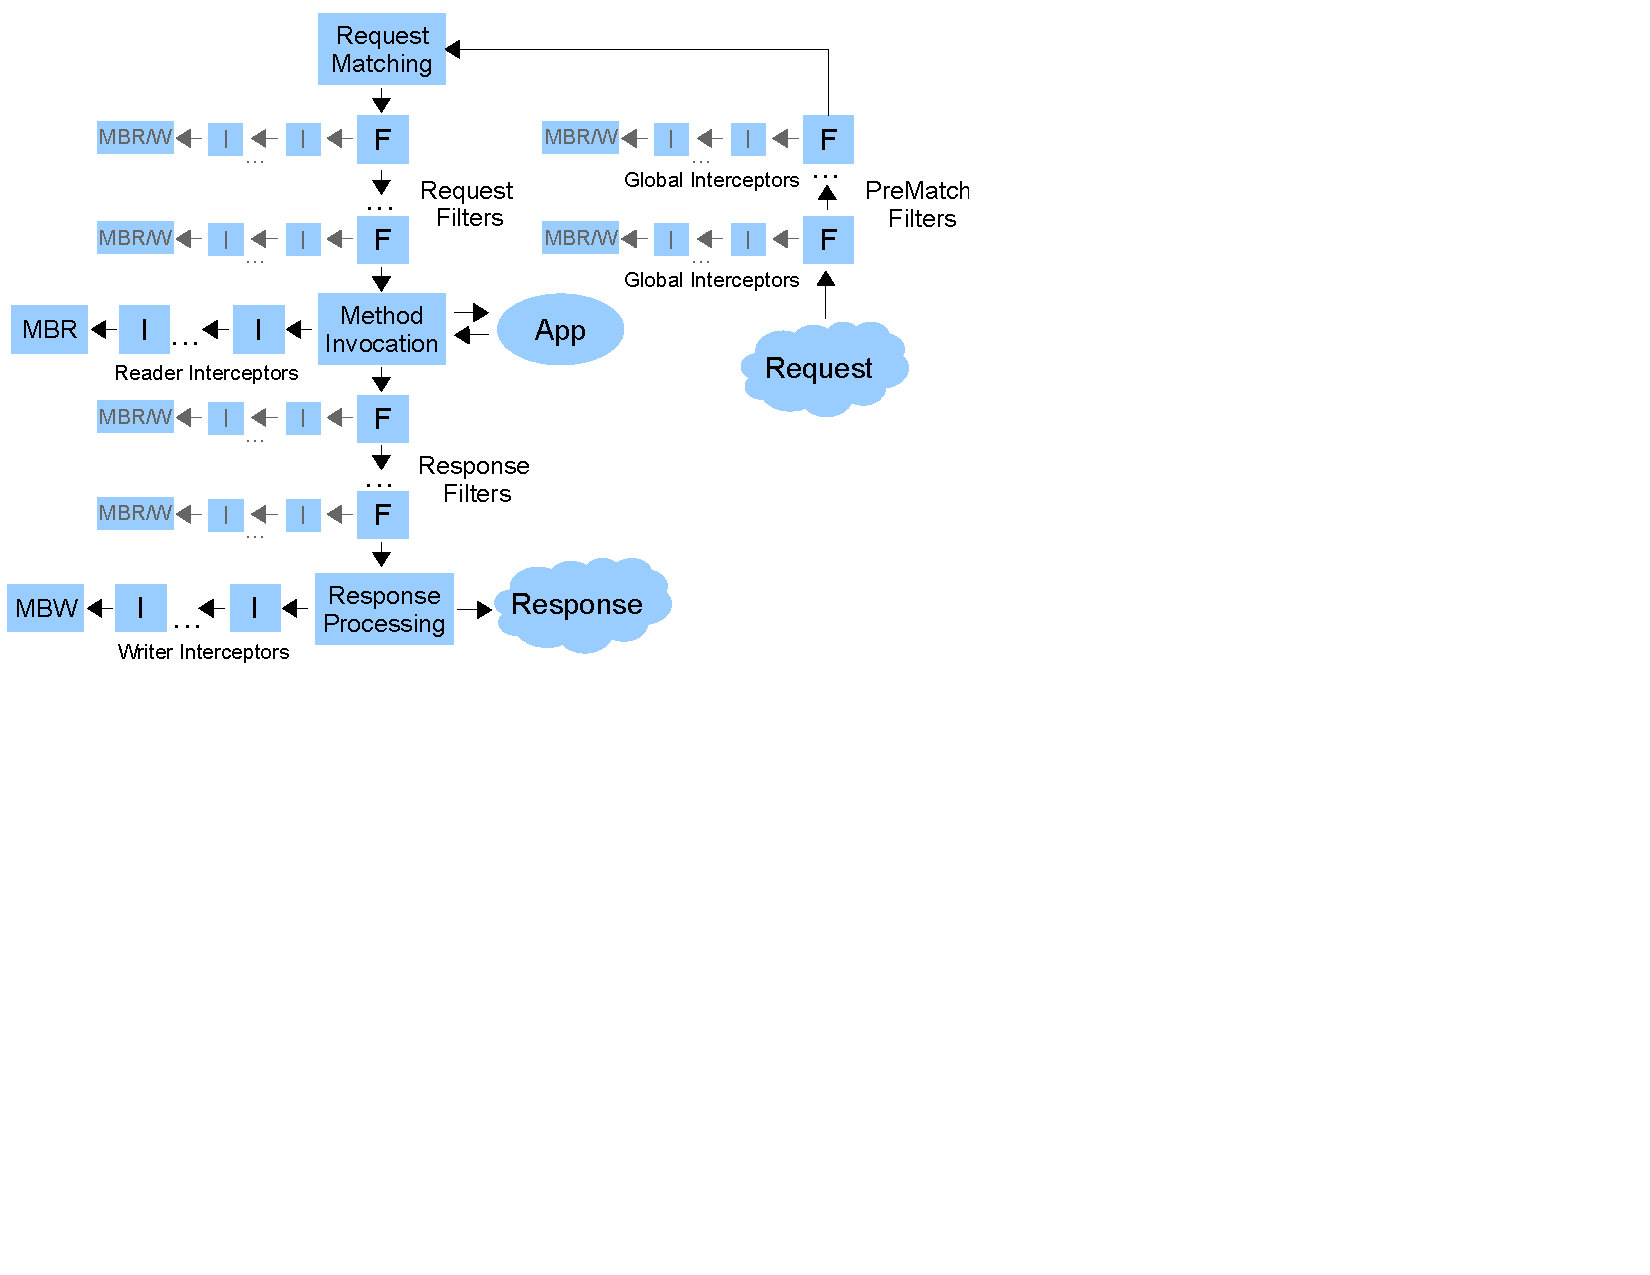
\includegraphics{chapters/jaxrs_pipeline.pdf}
\caption{JAX-RS Server Processing Pipeline.}
\label{jaxrs_pipeline}
\end{figure}

